\documentclass[12pt, a4paper]{article}

% --- CORE & TYPOGRAPHY PACKAGES ---
\usepackage[margin=1in]{geometry}
\usepackage{microtype}
\usepackage{xcolor}
\definecolor{amber}{RGB}{255, 191, 0}
\usepackage{hyperref}
\hypersetup{colorlinks=true, linkcolor=blue, urlcolor=cyan}

% --- MATHEMATICS ---
% Load physics BEFORE amsmath/mathtools to prevent command collisions
\usepackage{physics}
\usepackage{amsmath, amsfonts, amssymb, amsthm}
\usepackage{mathtools}

% --- GRAPHICS & EXTERNAL PACKAGES ---
\usepackage{tikz}
\usepackage{tikz-cd}
\usetikzlibrary{shapes, arrows.meta, positioning, calc}

\usepackage{pgfplots}
\pgfplotsset{compat=1.18}

% Asymptote (Requires 'asy' processing pipeline)
\usepackage{asymptote}

% Chemistry & Science
\usepackage[version=4]{mhchem}
\usepackage{chemfig}

% --- TABLES & BOXES ---
\usepackage{booktabs}
\usepackage{multirow}
\usepackage{tabularx}
\usepackage[most]{tcolorbox}

% --- CODE LISTINGS ---
\usepackage{listings}
\lstset{
  basicstyle=\ttfamily\small,
  keywordstyle=\color{blue}\bfseries,
  commentstyle=\color{gray}\itshape,
  stringstyle=\color{red},
  breaklines=true,
  frame=single
}

% --- CUSTOM MACRO DEFINITIONS ---
\newcommand{\tensor}[1]{\mathbf{#1}}
\newcommand{\R}{\mathbb{R}}
\newcommand{\C}{\mathbb{C}}
\newcommand{\Laplace}{\mathcal{L}}

\title{\textbf{LaTeX Renderer Ultimate Benchmark Suite}}
\author{Real-Time Engine Stress Test}
\date{\today}

\begin{document}

\maketitle
\tableofcontents
\newpage

% ==========================================
% SECTION 1: TYPOGRAPHY & MACROS
% ==========================================
\section{Typography, Macros, \& Hyperlinks}
Testing basic text formatting, custom macro expansions, and hyper-referencing.

\begin{itemize}
  \item \textbf{Macro Expansion Test:} Let $x \in \R^n$ and $z \in \C$.
  \item \textbf{Inline Math:} The famous Euler identity is $e^{i\pi} + 1 = 0$, while the Gaussian integral evaluates to $\int_{-\infty}^{\infty} e^{-x^2} dx = \sqrt{\pi}$ and also $\frac{3}{4}$.
  \item \textbf{Interactive Link:} Visit \url{https://latex-project.org} or inspect Section \ref{sec:math}.
\end{itemize}

% ==========================================
% SECTION 2: COMPLEX MATH & MATRICES
% ==========================================
\section{Complex Mathematics \& Matrices}\label{sec:math}
Testing equation aligning, multi-line brackets, matrices, and commutative diagrams.

\subsection{Navier-Stokes \& Relativistic Physics}
\begin{align}
    \rho \left( \frac{\partial \mathbf{u}}{\partial t} + \mathbf{u} \cdot \nabla \mathbf{u} \right) &= -\nabla p + \mu \nabla^2 \mathbf{u} + \mathbf{f} \label{eq:navier} \\
    R_{\mu\nu} - \frac{1}{2}R g_{\mu\nu} + \Lambda g_{\mu\nu} &= \frac{8\pi G}{c^4} T_{\mu\nu}
\end{align}

\subsection{Deeply Nested Matrices \& Multi-alignment}
\[
\begin{pmatrix}
\frac{\partial^2 f}{\partial x_1^2} & \frac{\partial^2 f}{\partial x_1 \partial x_2} & \cdots & \frac{\partial^2 f}{\partial x_1 \partial x_n} \\
\frac{\partial^2 f}{\partial x_2 \partial x_1} & \frac{\partial^2 f}{\partial x_2^2} & \cdots & \frac{\partial^2 f}{\partial x_2 \partial x_n} \\
\vdots & \vdots & \ddots & \vdots \\
\frac{\partial^2 f}{\partial x_n \partial x_1} & \frac{\partial^2 f}{\partial x_n \partial x_2} & \cdots & \frac{\partial^2 f}{\partial x_n^2}
\end{pmatrix}
\cdot 
\begin{bmatrix}
v_1 \\ v_2 \\ \vdots \\ v_n
\end{bmatrix}
=
\begin{Bmatrix}
\lambda_1 \\ \lambda_2 \\ \vdots \\ \lambda_n
\end{Bmatrix}
\]

\subsection{Category Theory (TikZ-CD)}
\begin{tikzcd}
T \arrow[dr, "y"'] \arrow[r, "x"] \arrow[rr, "h", bend right=20] & X \arrow[d, "f"] \arrow[r, "g"] & Y \arrow[d, "q"] \\
& Z \arrow[r, "p"'] & W
\end{tikzcd}

% ==========================================
% SECTION 3: 2D VECTOR GRAPHICS
% ==========================================
\section{2D Vector Graphics \& Function Plotting}

\begin{figure}[h]
\centering
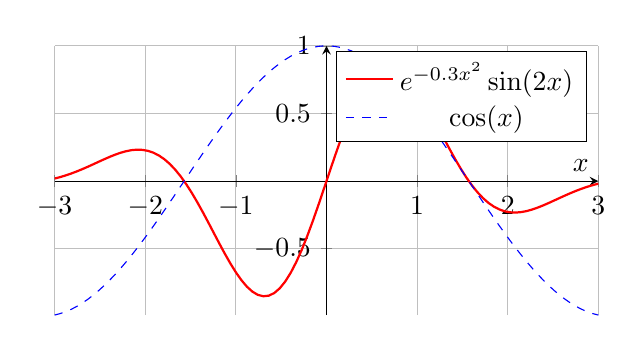
\begin{tikzpicture}
\begin{axis}[
    axis lines = middle,
    xlabel = $x$,
    ylabel = {$f(x)$},
    domain = -3:3,
    samples = 100,
    grid = major,
    width=0.7\textwidth,
    height=5cm
]
\addplot [red, thick] {sin(deg(x)*2) * exp(-0.3*x^2)};
\addlegendentry{$e^{-0.3x^2} \sin(2x)$}
\addplot [blue, dashed] {cos(deg(x))};
\addlegendentry{$\cos(x)$}
\end{axis}
\end{tikzpicture}
\caption{PGFPlots Dynamic Function Plotting}
\end{figure}

% ==========================================
% SECTION 4: 3D GRAPHICS BENCHMARK
% ==========================================
\section{3D Vector Graphics \& Surface Rendering}

\subsection{PGFPlots: 3D Parametric Surface Mesh}
\begin{figure}[h]
\centering
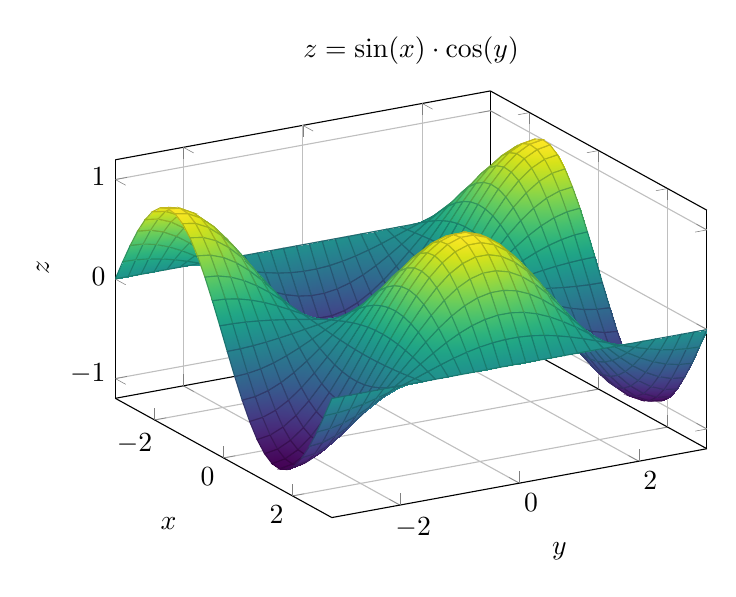
\begin{tikzpicture}
\begin{axis}[
    title={$z = \sin(x) \cdot \cos(y)$},
    xlabel=$x$, ylabel=$y$, zlabel=$z$,
    colormap/viridis,
    view={60}{30},
    width=0.75\textwidth,
    height=7cm,
    grid=major
]
\addplot3[
    surf,
    shader=faceted interp,
    domain=-3.14:3.14,
    domain y=-3.14:3.14,
    samples=30
] {sin(deg(x)) * cos(deg(y))};
\end{axis}
\end{tikzpicture}
\caption{PGFPlots 3D Surface Interpolation}
\end{figure}

\subsection{Asymptote: 3D Vector Geometry \& Transparency}
\begin{asy}
import three;
import graph3;

size(8cm, 0);
currentprojection = perspective(camera=(5, 4, 3), target=(0,0,0));

// 3D Coordinate Axes
draw(O--1.5*X, red + 1pt, Arrow3());
draw(O--1.5*Y, green + 1pt, Arrow3());
draw(O--1.5*Z, blue + 1pt, Arrow3());

label("$x$", 1.6*X, red);
label("$y$", 1.6*Y, green);
label("$z$", 1.6*Z, blue);

// 3D Parametric Helix
triple helix(real t) {
    return (cos(t), sin(t), t / 5);
}

path3 myHelix = graph(helix, 0, 4*pi, operator ..);
draw(myHelix, heavycyan + 1.5pt);

// Semi-transparent 3D Sphere shell
draw(unitsphere, opacity(0.25) + lightgray);

// Point along the helix
dot(helix(3*pi), red + 4pt);
\end{asy}

% ==========================================
% SECTION 5: 2D ASYMPTOTE GRAPHICS
% ==========================================
\section{External Package Integration: 2D Asymptote}

\begin{asy}
size(6cm, 0);
import graph;

xlimits(-2, 2);
ylimits(-2, 2);
xaxis("$x$", Arrow);
yaxis("$y$", Arrow);

draw(unitcircle, blue + linewidth(1pt));
draw((0,0)--(cos(pi/4), sin(pi/4)), red + dashed);
label("$r = 1$", (0.4, 0.2), red);
dot((cos(pi/4), sin(pi/4)), green);
\end{asy}

% ==========================================
% SECTION 6: CHEMISTRY
% ==========================================
\section{Chemistry \& Molecular Structures}

\subsection{Inorganic Reactions (mhchem)}
\ce{2KMnO4 + 16HCl -> 2MnCl2 + 2KCl + 5Cl2 ^ + 8H2O}

\subsection{Organic Molecules (chemfig)}
\begin{center}
\chemfig{*6(=-=-=-)}
\quad
\chemfig{A-[:30]B=[:-30]C-[:30]D}
\end{center}

% ==========================================
% SECTION 7: STYLED CONTAINERS, TABLES \& CODE
% ==========================================
\section{Styled Containers, Tables \& Code Listings}

\begin{tcolorbox}[colback=blue!5!white, colframe=blue!75!black, title=\textbf{Real-Time Render Target}]
This box tests custom block shadows, border radii, and background blending along with embedded formulas:
\[
\oint_C \mathbf{E} \cdot d\mathbf{l} = -\frac{\partial}{\partial t} \iint_S \mathbf{B} \cdot d\mathbf{S}
\]
\end{tcolorbox}

\subsection{Advanced Table Layout (TabularX + Booktabs)}
\begin{table}[h]
\centering
\begin{tabularx}{\textwidth}{l X r c}
\toprule
\textbf{Module} & \textbf{Rendering Strategy} & \textbf{Complexity} & \textbf{Status} \\
\midrule
Math Engine & AST Parsing to Canvas/SVG & $\mathcal{O}(N)$ & \textcolor{green!60!black}{\textbf{PASS}} \\
TikZ 2D/3D  & Vector Path Compilation & $\mathcal{O}(N^2)$ & \textcolor{green!60!black}{\textbf{PASS}} \\
Asymptote   & Asynchronous Subprocess Pipe & $\mathcal{O}(\text{Process})$ & \textcolor{amber}{\textbf{PENDING}} \\
\bottomrule
\end{tabularx}
\end{table}

\subsection{Code Listings}
\begin{lstlisting}[language=C++]
// Memory stress test loop for render tree validation
#include <iostream>

template<typename T>
T fast_render(T input) {
    return input * 1.61803398875; // Golden Ratio scaling
}
\end{lstlisting}

\end{document}
